\section{Controlling the DC motor from OpenModelica}
\subsection{Controlling the DC motor}
In this section, we discuss how to carry out the experiments of the
previous section from OpenModelica.  We will list the same three experiments,
in the same order.  As mentioned earlier, the Shield must be removed from 
the \arduino\ and the \arduino\ needs to be connected to the computer 
with a USB cable, as shown in \figref{arduino}. The reader should go through the instructions given in
\secref{sec:OpenModelica-start} before getting started.



\paragraph{Note:} The readers are advised to affix a small 
(very lightweight) piece of paper at the tip of the shaft of the DC motor. 
That will help them observe the direction of rotation 
of the DC motor while running the experiments.

\begin{enumerate}
  \item In the first experiment, we will learn how to drive the DC motor
        from OpenModelica. The code for this experiment is 
        given in  \OpenModelicaref{OpenModelica:dcmotor-clock}. 
        As explained earlier in \secref{sec:light-OpenModelica}, 
        we begin with importing the two packages: Streams and SerialCommunication followed 
        by setting up the serial port. Next, the code has a command of the following form: 
        \begin{lstlisting}[style=nonumbers]
          cmd_dcmotor_setup(1, H-Bridge type, Motor number, PWM pin 1, PWM pin 2)
        \end{lstlisting}
        As mentioned earlier, this chapter makes use of an H-Bridge circuit which 
        allows direction of the current passing through the DC motor to be changed.
        We are using L293D as an H-Bridge circuit in this book. Thus, we will pass the value 3 for
        H-Bridge type. OpenModelica-Arduino toolbox, as explained in 
        \secref{sec:load-om-toolbox}, 
        supports three types of H-Bridge circuit. \tabref{table:convention}
        provides the values to be passed for different H-Bridge circuits. 
        Next argument in the command given above is Motor number. Here, we pass the value 1. 
        Finally, we provide the PWM pins to which the DC motor is connected. As 
        shown in \figref{fig:dcmotorconn}, pins 9 and 10 are connected to the
        input of the breakout board. As a result, the command {\tt cmd\_dcmotor\_setup} becomes
        \lstinputlisting[firstline=15,lastline=15]
        {\LocDCMOpenModelicacode/dcmotor-clock.mo}
        
        The next line of \OpenModelicaref{OpenModelica:dcmotor-clock} is of the following form: 
        \begin{lstlisting}[style=nonumbers]
          cmd_dcmotor_run(1, Motor number, [sign] PWM value)
        \end{lstlisting}
        Here, we will pass the value 1 in Motor number.  As mentioned earlier, 
        for each of the PWM pins on \arduino\ board, the input can come from 8 bits.
        Thus, these pins can supply values between $- 255$ and $+ 255$. Positive values correspond to clockwise
        rotation while negative values correspond to anti-clockwise rotation. Based on the PWM value and polarity, 
        corresponding analog voltage is generated.  
        We put a PWM value of 100 to make the DC motor run at an intermediate speed.  
        As a result, the command {\tt cmd\_dcmotor\_run} becomes
        \lstinputlisting[firstline=16,lastline=16]
        {\LocDCMOpenModelicacode/dcmotor-clock.mo}
        
        The above-mentioned command does not say for how long the motor should run.  This is taken care of
        by the {\tt sleep} command, as given below:
        \lstinputlisting[firstline=17,lastline=17]{\LocDCMOpenModelicacode/dcmotor-clock.mo}
        With this, the DC motor will run for 3000 milliseconds or 3 seconds. At last, 
        we release the DC motor, as shown below:
        \lstinputlisting[firstline=18,lastline=18]{\LocDCMOpenModelicacode/dcmotor-clock.mo}
        With the execution of this command, the PWM functionality on the \arduino\ pins
        is ceased.  This has the motor number as an input
        parameter. At last, we close the serial port. 
        
        \paragraph{Note:} If the sleep command (at line 17 of \OpenModelicaref{OpenModelica:dcmotor-clock}) 
        were not present, the DC motor will not even run: soon after putting the value 100, 
        the DC motor would be released, leaving no time in between.  On the other hand, if
        the DC motor is not released (\ie\ line number 18 of \OpenModelicaref{OpenModelica:dcmotor-clock} being commented), 
        the DC motor will go on rotating. That's why, it may be inferred that 
        line number 18 of \OpenModelicaref{OpenModelica:dcmotor-clock} is mandatory
        for every program. We encourage the readers to run  \OpenModelicaref{OpenModelica:dcmotor-clock} by commenting
        any one or two of the lines numbered 17 and 18.  Go ahead and do it - you will not break
        anything.  At the most, you may have to unplug the USB cable connected to \arduino\ and
        restart the whole thing from the beginning.
        
  \item It is easy to make the DC motor run in the reverse direction by
        changing the sign of PWM value being written.  This is done in
        \OpenModelicaref{OpenModelica:dcmotor-both}.  In this code, we make the DC motor
        run in one direction for 3 seconds and then make it rotate in the
        reverse direction for 2 seconds.  The rotation in reverse direction
        is achieved by putting $- 100$ in the command {\tt cmd\_dcmotor\_run}, 
        as shown below:
        \lstinputlisting[firstline=17,lastline=17]
        {\LocDCMOpenModelicacode/dcmotor-both.mo}
        % This makes the green LED light up as well, recall the discussion in \secref{sec:led-pril}.  After
        After adding a {\tt sleep} of 2 seconds, we release the motor by issuing
        the command {\tt cmd\_dcmotor\_release}, followed by closing the serial port:
        \lstinputlisting[firstline=19,lastline=19]
        {\LocDCMOpenModelicacode/dcmotor-both.mo}
        With this, the motor comes to a halt.  
        % This turns the green LED off as well.
        
  \item Next, we make the DC motor run in forward and reverse
        directions, in a loop.  This is done through
        \OpenModelicaref{OpenModelica:dcmotor-loop}.  We first write PWM $+100$ for 3
        seconds.  After that, halt the motor for 2 seconds by writing zero PWM value.  
        Next, make the motor rotate in the reverse direction by writing PWM $-100$ for two seconds.  
        Next, we make the motor stop for one second. This procedure is put in a {\tt for} loop which runs for 4 iterations.
        At last, we release the motor by issuing the command {\tt cmd\_dcmotor\_release}, followed by closing the serial port. 
        
\end{enumerate}



%%%%%%%OpenModelica description ends

% \subsection{Using the Xcos features in DC motor control}
% Xcos can be used to control the DC motor in many different ways.  In
% this section, we will see a few approaches.  First, we will make the
% DC motor start and stop.  For this, we will open the program given in \figref{fig:dcm-xcos-start-stop}.
% \begin{figure}
% \centering
% 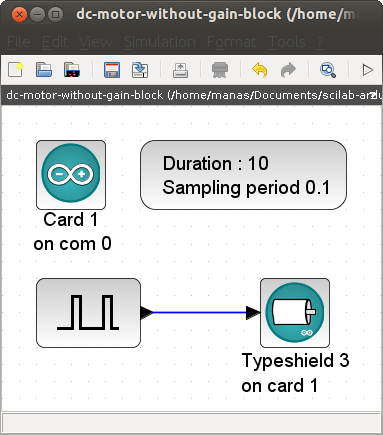
\includegraphics[width=\smfig]{\LocDCMfig/dc-motor-start-stop.png}
% \caption[Xcos program to make the DC motor to rotate, pause and
%   repeat]{Xcos program to make the DC motor to rotate, pause and
%   repeat.  This is what one sees when {\tt
%     \LocDCMscibrief/dc-motor-start-stop.zcos} is invoked.}
% \label{fig:dcm-xcos-start-stop}
% \end{figure}

% The input is a train of pulses of positive values.  The amplitude of
% these pulses is chosen to be 255.  The period is chosen to be 1s.
% \redcolor{these values have to be checked - this section to be
%   rewritten.}  On executing this Xcos code, the DC motor rotates for
% 1s, pauses for 1s, and repeats.  This continues until the Xcos program
% is terminated.

% \begin{exercise}
% Carry out the following exercise:
% \begin{enumerate}
% \item The user may repeat this exercise with different amplitude and
%   periods. 
% \item The above may be repeated with negative PWM values.
% \item One may find the least count for all experiments.
% \end{enumerate}
% \end{exercise}

% We will next see how to give positive and negative values of PWM in
% the same experiment.  For this, we will use the Xcos program given in
% \figref{fig:dcm-xcos-both}.  This code is similar to the previous one,
% but for a few minor changes.  First of all, we have introduced a gain
% block, and assigned a value of 255.  This block is excited by pulses
% of $+1$ and $-1$ alternately.  This simple approach, however, results
% in the DC motor running in both directions for identical durations.
% \begin{figure}
% \centering
% 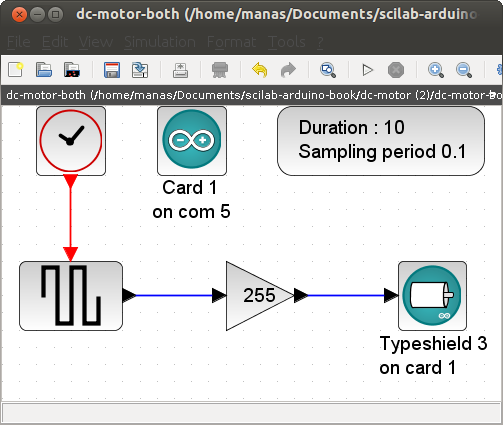
\includegraphics[width=\lgfig]{\LocDCMfig/dc-motor-both.png}
% \caption[Xcos program to make the DC motor to rotate, pause and to
%   rotate in the opposite direction]{Xcos program to make the DC motor
%   to rotate, pause and to rotate in the opposite direction.  This is
%   what one sees when {\tt \LocDCMscibrief/dc-motor-both.zcos} is
%   invoked.}
% \label{fig:dcm-xcos-both}
% \end{figure}

% \begin{exercise}
% Carry out the following exercise:
% \begin{enumerate}
% \item Repeat this experiment for different amplitudes and periods.
% \end{enumerate}
% \end{exercise}


% \subsection{Troubleshooting \redcolor{Do we need this? - Manas, please answer}}
% \begin{enumerate}
% \item If we want to connect external supply, Ground (Gnd) pin of L293D board, external supply and \arduino\ board should be shorted. This creates common ground voltage for entire set-up.
% \item We can connect more than one motor simultaneously using H-bridge like L293D. Typically break-out boards support 2 motors. However we are limited by number of PWM pins available on the board. For each motor cable of bidirectional motion, we need two PWM pins
% \end{enumerate}


\subsection{OpenModelica Code}
\label{sec:dcmotor-OpenModelica-code}
Unlike other code files, the code/model for running experiments using OpenModelica are 
available inside OpenModelica-Arduino toolbox, as explained in \secref{sec:load-om-toolbox}.
Please refer to \figref{om-examples-toolbox} to know how to locate the experiments. 

\addtocontents{OpenModelicad}{\protect\addvspace{\codclr}}

\begin{OpenModelicacode}
  \mcaption{Rotating the DC motor}
  {Rotating the DC motor.  
  Available at Arduino -> SerialCommunication -> Examples -> dcmotor 
    -> dcmotor\_clock.}
  \label{OpenModelica:dcmotor-clock}
  \lstinputlisting{\LocDCMOpenModelicacode/dcmotor-clock.mo}
\end{OpenModelicacode}

\begin{OpenModelicacode}
  \mcaption{Rotating the DC motor in both directions}
  {Rotating DC motor in both directions.  Available at Arduino -> SerialCommunication -> Examples -> dcmotor 
    -> dcmotor\_both.}
  \label{OpenModelica:dcmotor-both}
  \lstinputlisting{\LocDCMOpenModelicacode/dcmotor-both.mo}
\end{OpenModelicacode}

\begin{OpenModelicacode}
  \mcaption{Rotating the DC motor in both directions in a loop}{Rotating
    the DC motor in both directions in a loop.
    Available at Arduino -> SerialCommunication -> Examples -> dcmotor 
    -> dcmotor\_loop.}
  \label{OpenModelica:dcmotor-loop}
  \lstinputlisting{\LocDCMOpenModelicacode/dcmotor-loop.mo}
\end{OpenModelicacode}
%%%%%%%%%%OpenModelica code ends
